\documentclass[a4paper, 12pt, final, garamond]{book}
\usepackage{cours-preambule}

\raggedbottom

\makeatletter
\renewcommand{\@chapapp}{Programme de kh\^olle -- semaine}
\makeatother

\begin{document}
\setcounter{chapter}{1}

\chapter{Du 19 au 23 septembre}
\section*{Exercice de cours~: champ de vision à travers un miroir plan}

Une personne dont les yeux se situent à $h = \SI{1.70}{m}$ du sol observe une
mare gelée (équivalente à un miroir plan) de largeur $l = \SI{5.00}{m}$ et
située à $d = \SI{2.00}{m}$ d'elle.

\begin{enumerate}
    \item Peut-elle voir sa propre image~? Quelle est la nature de l'image~?
    \item Quelle est la hauteur maximale $H$ d'un arbre situé de l'autre côté de
        la mare (en bordure de mare) qu'elle peut voir par réflexion dans la
        mare~? On notera $D = l+d$.
\end{enumerate}

\subsection{Propre image}
\begin{NCdefi}{Schéma}
    \begin{center}
        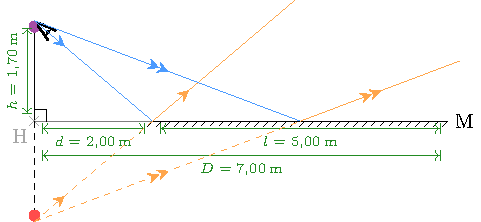
\includegraphics[width=\linewidth]{ch3-arbre-1}
    \end{center}
\end{NCdefi}
\begin{tcbraster}[raster columns=2, raster equal height=rows]
    \begin{NCrapp}{Outil}
        Pour voir une image, il faut qu'un rayon partant de l'image
        puisse arriver jusqu'à l'œil de l'observataire. Étant donné
        qu'on travaille avec un miroir, l'image de l'observataire est
        son symétrique par le plan du miroir (même si le miroir ne
        s'étend pas jusque-là !).
    \end{NCrapp}
    \begin{NCexem}{Application}
        On voit vite qu'il n'est pas possible qu'un rayon issu de
        l'image (en rouge) atteigne l'œil (en violet). On comprend par
        le tracé des rayons réfléchis que seul l'autre côté du lac sera
        visible.
    \end{NCexem}
\end{tcbraster}

\subsection{Image arbre}
\begin{NCdefi}{Schéma}
    \begin{center}
        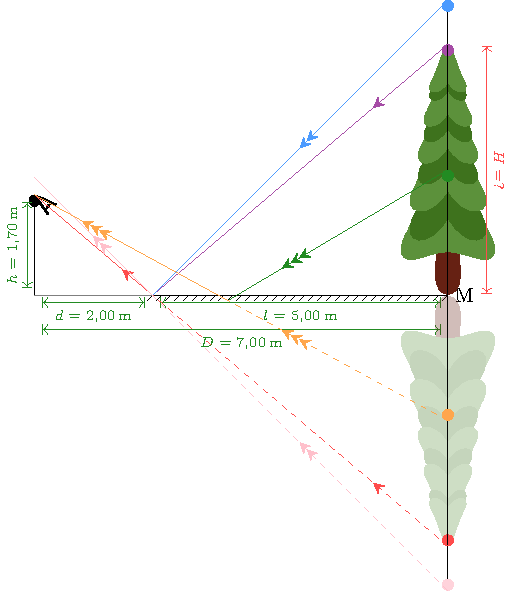
\includegraphics[width=.7\linewidth]{ch3-arbre-2}
    \end{center}
\end{NCdefi}
\begin{NCrapp}[]{Outil}
    Ici aussi, l'idée est de trouver l'image de l'arbre, et de voir
    la condition limite pour la taille visible.
\end{NCrapp}
\begin{NCexem}{Application}
    Un schéma avec l'image de l'arbre nous permet de voir que le
    point le plus haut qu'on peut voir par réflexion sur le lac est
    quand on regarde proche de nous : si on regarde plus loin, on
    voit en effet plus vers le bas de l'arbre (rayon vert incident,
    rayon orange émergent). Un arbre qui est trop grand ne sera pas
    visible en regardant ce point-là (rayon bleu incident, rose
    émergent). On s'intéresse donc à la construction géométrique
    formée par le rayon violet incident, rouge émergent, qui nous
    permet d'appliquer le théorème de Thalès : $\DS\frac{H}{l} =
    \frac{h}{d}$, soit
    \[\boxed{H = \frac{l\times h}{d}} \quad \text{avec} \quad
        \left\{
            \begin{array}{rcl}
                l & = & \SI{5.00}{m}\\
                h & = & \SI{1.70}{m}\\
                d & = & \SI{2.00}{m}
            \end{array}
    \right.\]
    D'où
    \[\boxed{H = \SI{4.25}{m}}\]
\end{NCexem}

\end{document}
